\documentclass[]{article}
\usepackage{lmodern}
\usepackage{amssymb,amsmath}
\usepackage{ifxetex,ifluatex}
\usepackage{fixltx2e} % provides \textsubscript
\ifnum 0\ifxetex 1\fi\ifluatex 1\fi=0 % if pdftex
  \usepackage[T1]{fontenc}
  \usepackage[utf8]{inputenc}
\else % if luatex or xelatex
  \ifxetex
    \usepackage{mathspec}
  \else
    \usepackage{fontspec}
  \fi
  \defaultfontfeatures{Ligatures=TeX,Scale=MatchLowercase}
\fi
% use upquote if available, for straight quotes in verbatim environments
\IfFileExists{upquote.sty}{\usepackage{upquote}}{}
% use microtype if available
\IfFileExists{microtype.sty}{%
\usepackage{microtype}
\UseMicrotypeSet[protrusion]{basicmath} % disable protrusion for tt fonts
}{}
\usepackage[margin=1in]{geometry}
\usepackage{hyperref}
\hypersetup{unicode=true,
            pdftitle={DATA 621 - Homework 3},
            pdfauthor={Joshua Sturm},
            pdfborder={0 0 0},
            breaklinks=true}
\urlstyle{same}  % don't use monospace font for urls
\usepackage{graphicx,grffile}
\makeatletter
\def\maxwidth{\ifdim\Gin@nat@width>\linewidth\linewidth\else\Gin@nat@width\fi}
\def\maxheight{\ifdim\Gin@nat@height>\textheight\textheight\else\Gin@nat@height\fi}
\makeatother
% Scale images if necessary, so that they will not overflow the page
% margins by default, and it is still possible to overwrite the defaults
% using explicit options in \includegraphics[width, height, ...]{}
\setkeys{Gin}{width=\maxwidth,height=\maxheight,keepaspectratio}
\IfFileExists{parskip.sty}{%
\usepackage{parskip}
}{% else
\setlength{\parindent}{0pt}
\setlength{\parskip}{6pt plus 2pt minus 1pt}
}
\setlength{\emergencystretch}{3em}  % prevent overfull lines
\providecommand{\tightlist}{%
  \setlength{\itemsep}{0pt}\setlength{\parskip}{0pt}}
\setcounter{secnumdepth}{0}
% Redefines (sub)paragraphs to behave more like sections
\ifx\paragraph\undefined\else
\let\oldparagraph\paragraph
\renewcommand{\paragraph}[1]{\oldparagraph{#1}\mbox{}}
\fi
\ifx\subparagraph\undefined\else
\let\oldsubparagraph\subparagraph
\renewcommand{\subparagraph}[1]{\oldsubparagraph{#1}\mbox{}}
\fi

%%% Use protect on footnotes to avoid problems with footnotes in titles
\let\rmarkdownfootnote\footnote%
\def\footnote{\protect\rmarkdownfootnote}

%%% Change title format to be more compact
\usepackage{titling}

% Create subtitle command for use in maketitle
\newcommand{\subtitle}[1]{
  \posttitle{
    \begin{center}\large#1\end{center}
    }
}

\setlength{\droptitle}{-2em}
  \title{DATA 621 - Homework 3}
  \pretitle{\vspace{\droptitle}\centering\huge}
  \posttitle{\par}
  \author{Joshua Sturm}
  \preauthor{\centering\large\emph}
  \postauthor{\par}
  \predate{\centering\large\emph}
  \postdate{\par}
  \date{04/02/2018}

\usepackage{booktabs}
\usepackage{longtable}
\usepackage{array}
\usepackage{multirow}
\usepackage[table]{xcolor}
\usepackage{wrapfig}
\usepackage{float}
\usepackage{colortbl}
\usepackage{pdflscape}
\usepackage{tabu}
\usepackage{threeparttable}
\usepackage[normalem]{ulem}

\begin{document}
\maketitle

\section{Introduction}\label{introduction}

Your objective is to build a binary logistic regression model on the
training data set to predict whether the neighbourhood will be at risk
for high crime levels. You will provide classifications and
probabilities for the evaluation data set using your binary logistic
regression model. You can only use the variables given to you (or,
variables that you derive from the variables provided).

\section{1. Data Exploration}\label{data-exploration}

\subsection{1.1 Load Libraries}\label{load-libraries}

\subsection{1.2 Read in data}\label{read-in-data}

\subsubsection{1.2.1 Create data
dictionary}\label{create-data-dictionary}

\begin{table}[H]
\centering\rowcolors{2}{gray!6}{white}

\resizebox{\linewidth}{!}{\begin{tabular}{lll}
\hiderowcolors
\toprule
Variable Name & Definition & NA\\
\midrule
\showrowcolors
zn & proportion of residential land zoned for large lots (over 25000 square feet) & Outcome variable\\
indus & proportion of non-retail business   acres per suburb & Outcome variable\\
chas & a dummy var. for whether the suburb borders the Charles River (1) or not (0) & Outcome variable\\
nox & nitrogen oxides concentration (parts per 10 million) & Outcome variable\\
rm & average number of rooms per dwelling & Outcome variable\\
\addlinespace
age & proportion of owner-occupied units built prior to 1940 & Outcome variable\\
dis & weighted mean of distances to five Boston employment centers & Outcome variable\\
rad & index of accessibility to radial highways & Outcome variable\\
tax & full-value property-tax rate per \$10,000 & Outcome variable\\
ptratio & pupil-teacher ratio by town & Outcome variable\\
\addlinespace
lstat & lower status of the population (percent) & Outcome variable\\
medv & median value of owner-occupied homes in \$1000s & Outcome variable\\
\bottomrule
\end{tabular}}
\rowcolors{2}{white}{white}
\end{table}

\subsection{1.3 Basic dataset
statistics}\label{basic-dataset-statistics}

\begin{table}[H]
\centering\rowcolors{2}{gray!6}{white}

\resizebox{\linewidth}{!}{\begin{tabular}{lrrrrrrrrrrrrr}
\hiderowcolors
\toprule
  & vars & n & mean & sd & median & trimmed & mad & min & max & range & skew & kurtosis & se\\
\midrule
\showrowcolors
zn & 1 & 466 & 11.5772532 & 23.3646511 & 0.00000 & 5.3542781 & 0.0000000 & 0.0000 & 100.0000 & 100.0000 & 2.1768152 & 3.8135765 & 1.0823466\\
indus & 2 & 466 & 11.1050215 & 6.8458549 & 9.69000 & 10.9082353 & 9.3403800 & 0.4600 & 27.7400 & 27.2800 & 0.2885450 & -1.2432132 & 0.3171281\\
chas & 3 & 466 & 0.0708155 & 0.2567920 & 0.00000 & 0.0000000 & 0.0000000 & 0.0000 & 1.0000 & 1.0000 & 3.3354899 & 9.1451313 & 0.0118957\\
nox & 4 & 466 & 0.5543105 & 0.1166667 & 0.53800 & 0.5442684 & 0.1334340 & 0.3890 & 0.8710 & 0.4820 & 0.7463281 & -0.0357736 & 0.0054045\\
rm & 5 & 466 & 6.2906738 & 0.7048513 & 6.21000 & 6.2570615 & 0.5166861 & 3.8630 & 8.7800 & 4.9170 & 0.4793202 & 1.5424378 & 0.0326516\\
\addlinespace
age & 6 & 466 & 68.3675966 & 28.3213784 & 77.15000 & 70.9553476 & 30.0226500 & 2.9000 & 100.0000 & 97.1000 & -0.5777075 & -1.0098814 & 1.3119625\\
dis & 7 & 466 & 3.7956929 & 2.1069496 & 3.19095 & 3.5443647 & 1.9144814 & 1.1296 & 12.1265 & 10.9969 & 0.9988926 & 0.4719679 & 0.0976026\\
rad & 8 & 466 & 9.5300429 & 8.6859272 & 5.00000 & 8.6978610 & 1.4826000 & 1.0000 & 24.0000 & 23.0000 & 1.0102788 & -0.8619110 & 0.4023678\\
tax & 9 & 466 & 409.5021459 & 167.9000887 & 334.50000 & 401.5080214 & 104.5233000 & 187.0000 & 711.0000 & 524.0000 & 0.6593136 & -1.1480456 & 7.7778214\\
ptratio & 10 & 466 & 18.3984979 & 2.1968447 & 18.90000 & 18.5970588 & 1.9273800 & 12.6000 & 22.0000 & 9.4000 & -0.7542681 & -0.4003627 & 0.1017669\\
\addlinespace
lstat & 11 & 466 & 12.6314592 & 7.1018907 & 11.35000 & 11.8809626 & 7.0720020 & 1.7300 & 37.9700 & 36.2400 & 0.9055864 & 0.5033688 & 0.3289887\\
medv & 12 & 466 & 22.5892704 & 9.2396814 & 21.20000 & 21.6304813 & 6.0045300 & 5.0000 & 50.0000 & 45.0000 & 1.0766920 & 1.3737825 & 0.4280200\\
target & 13 & 466 & 0.4914163 & 0.5004636 & 0.00000 & 0.4893048 & 0.0000000 & 0.0000 & 1.0000 & 1.0000 & 0.0342293 & -2.0031131 & 0.0231835\\
\bottomrule
\end{tabular}}
\rowcolors{2}{white}{white}
\end{table}

The training data has 466 cases, with 13 predictor variables. Each case
represents a neighbourhood in Boston. Our large sample size satisfies
one of the requirements to fit our data to a logistic model.

Amazingly, there is not a single \texttt{NA} in the entire dataset,
which will make our data cleaning job much easier!

\subsection{1.4 Summary Graphs}\label{summary-graphs}

\subsubsection{1.4.1 Boxplot}\label{boxplot}

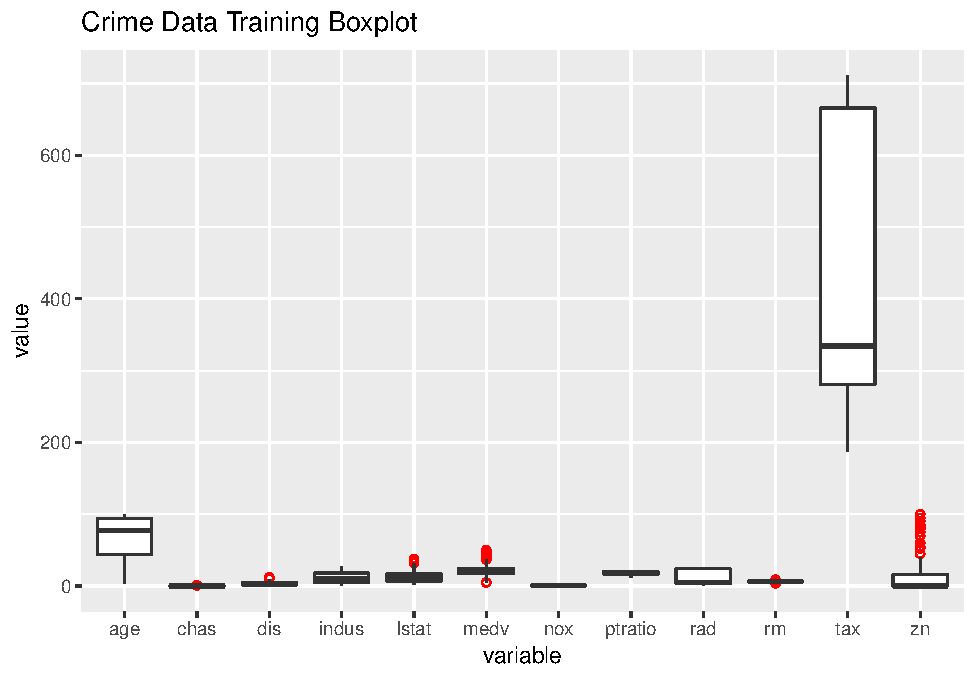
\includegraphics{DATA_621_Homework_3_files/figure-latex/summary-boxplot-1.pdf}

Aside from \texttt{zn}, this dataset doesn't have too many outliers.

\hypertarget{histogram}{\subsubsection{1.4.2
Histogram}\label{histogram}}

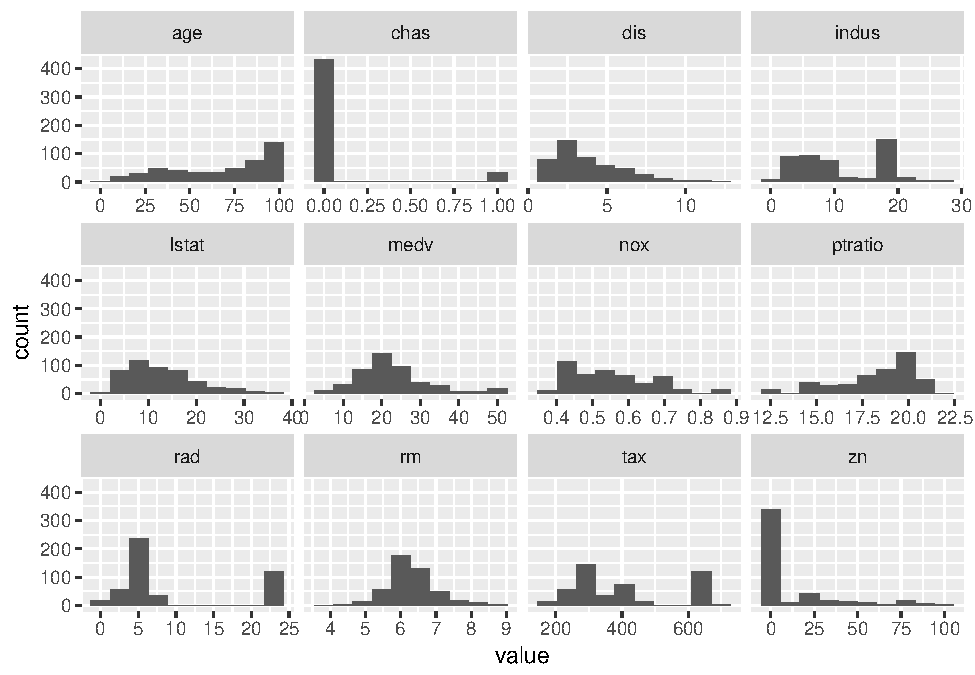
\includegraphics{DATA_621_Homework_3_files/figure-latex/summary-histogram-1.pdf}

We can see some variables, \texttt{age}, \texttt{chas}, \texttt{rad},
\texttt{zn}, in particular, are strongly skewed.

\subsubsection{1.4.3 Correlation}\label{correlation}

\paragraph{1.4.3.1 Correlation Heatmap}\label{correlation-heatmap}

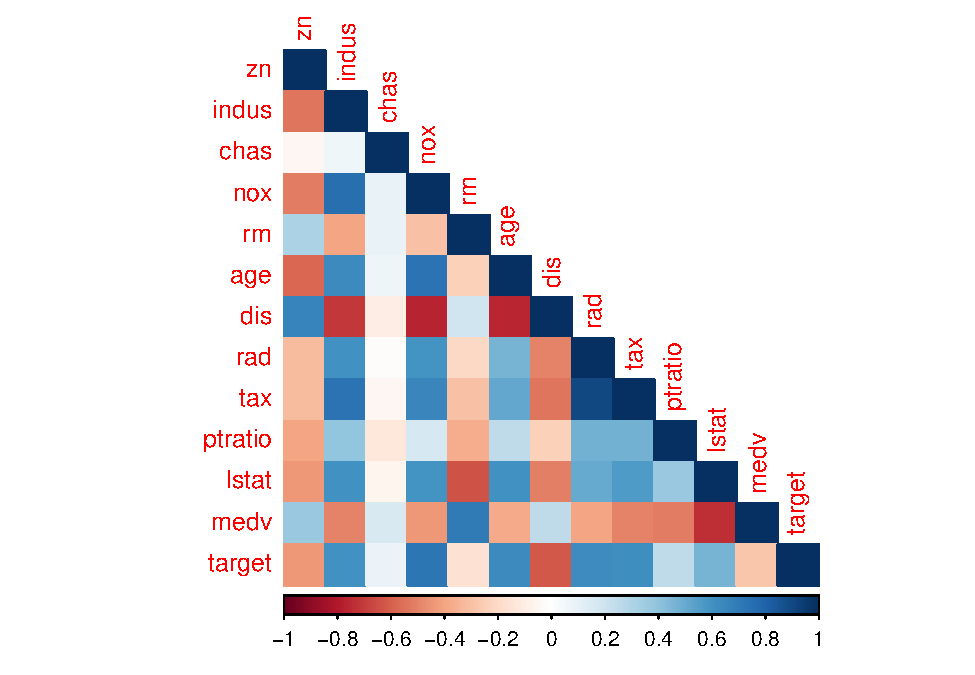
\includegraphics{DATA_621_Homework_3_files/figure-latex/summary-correlation-heatmap-1.pdf}

\paragraph{1.4.3.2 Correlation (with response)
table}\label{correlation-with-response-table}

\begin{table}[H]
\centering\rowcolors{2}{gray!6}{white}

\begin{tabular}{lll}
\hiderowcolors
\toprule
  & P-value & Correlation with response\\
\midrule
\showrowcolors
zn & 1.41560261828797e-22 & -0.431681757278317\\
indus & 7.84565111436042e-48 & 0.604850736249927\\
chas & 0.0843481072424482 & 0.0800418718031737\\
nox & 1.68013085953093e-77 & 0.726106218470473\\
rm & 0.00095422493976375 & -0.152553344896326\\
\addlinespace
age & 6.24573590524504e-53 & 0.63010624884034\\
dis & 1.4501758603908e-50 & -0.618673121688883\\
rad & 1.64759680001221e-52 & 0.628104918805408\\
tax & 4.70956558462997e-49 & 0.611113314858614\\
ptratio & 4.05273029910627e-08 & 0.250848917529503\\
\addlinespace
lstat & 7.07143116645425e-27 & 0.469127015198214\\
medv & 2.92493073681285e-09 & -0.270550708927679\\
\bottomrule
\end{tabular}
\rowcolors{2}{white}{white}
\end{table}

From the above correlation analysis, it appears that \texttt{chas} is
not correlated with neither the response variable, nor any of the other
predictor variables. This is important to note, since we may consider
removing it from the final model.

Another concern is the high correlation between \texttt{rad} and
\texttt{tax} - a staggering 0.9064632! We may want to remove one of
these predictors from our model to prevent muddying it with
collinearity.

\section{2. Data Preparation}\label{data-preparation}

\subsection{2.1 Missing Data}\label{missing-data}

As noted earlier, the dataset is remarkably whole, so we may proceed
without worrying about having to imputate any data.

\subsection{2.2 Normality of Predictor
Variables}\label{normality-of-predictor-variables}

As can be seen in the distribution plots in
\protect\hyperlink{histogram}{section 1.4.2}, many of the predictor
variables are not normally distributed. However, since logistic
regression makes no assumptions, including the normality of the
variables, we can safely skip this step, and keep the variables as they
are.

\subsection{2.3 Add or Remove Variables}\label{add-or-remove-variables}

As mentioned before, we'll consider removing two variables for one of
our models. \texttt{chas}, due to it's low correlation with any of the
other variables, and either \texttt{rad} or \texttt{tax}, due to high
collinearity between the two.

Other than the variables mentioned above, I don't see any reason to
remove any variables. Furthermore, there isn't enough implicit
information from which we could possibly derive new variables.

\hypertarget{variable-transformation}{\subsection{2.4 Variable
Transformation}\label{variable-transformation}}

339 of 466 cases in the \texttt{zn} variable have a value of 0, or
roughly 72.75\%. We may want to convert this to a binary variable, where

\[ zn = 
\begin{cases} 
      0 & zn = 0 \\
      1 & zn \neq 0
\end{cases}
\]

Additionally, we'll convert both the \texttt{target} variable, as well
as \texttt{chas}, from integers to factors.

\subsection{2.5 Outliers}\label{outliers}

I believe that once we recode the variable \texttt{zn} as outlined in
\protect\hyperlink{variable-transformation}{section 2.4}, we will no
longer have the outlier issue that is currently affecting the predictor.

\section{3. Build Models}\label{build-models}

Note that I will not be using any sort of `automatic' model selection,
e.g.~stepwise regression. After reading
\href{https://www.stata.com/support/faqs/statistics/stepwise-regression-problems/}{this
article}, I've decided to forego any automated choosing, and build (and
test) the models myself.

\subsection{3.1 Model 1}\label{model-1}

My first model will use the original dataset as is, without any variable
changes. This will serve as a sort of benchmark with which to gauge the
effectiveness of our changes.

\begin{verbatim}
## 
## Call:
## glm(formula = target ~ ., family = binomial(link = "logit"), 
##     data = crime.training)
## 
## Deviance Residuals: 
##     Min       1Q   Median       3Q      Max  
## -1.8464  -0.1445  -0.0017   0.0029   3.4665  
## 
## Coefficients:
##               Estimate Std. Error z value Pr(>|z|)    
## (Intercept) -40.822934   6.632913  -6.155 7.53e-10 ***
## zn           -0.065946   0.034656  -1.903  0.05706 .  
## indus        -0.064614   0.047622  -1.357  0.17485    
## chas1         0.910765   0.755546   1.205  0.22803    
## nox          49.122297   7.931706   6.193 5.90e-10 ***
## rm           -0.587488   0.722847  -0.813  0.41637    
## age           0.034189   0.013814   2.475  0.01333 *  
## dis           0.738660   0.230275   3.208  0.00134 ** 
## rad           0.666366   0.163152   4.084 4.42e-05 ***
## tax          -0.006171   0.002955  -2.089  0.03674 *  
## ptratio       0.402566   0.126627   3.179  0.00148 ** 
## lstat         0.045869   0.054049   0.849  0.39608    
## medv          0.180824   0.068294   2.648  0.00810 ** 
## ---
## Signif. codes:  0 '***' 0.001 '**' 0.01 '*' 0.05 '.' 0.1 ' ' 1
## 
## (Dispersion parameter for binomial family taken to be 1)
## 
##     Null deviance: 645.88  on 465  degrees of freedom
## Residual deviance: 192.05  on 453  degrees of freedom
## AIC: 218.05
## 
## Number of Fisher Scoring iterations: 9
\end{verbatim}

\subsubsection{3.1.1 Model 1
Interpretation}\label{model-1-interpretation}

There are several variables that are not significant to the model (i.e.
\(P > 0.05\)), including \texttt{indus}, \texttt{chas}, \texttt{rm},
\texttt{lstat}, with \texttt{zn} right on the border of 0.05.

\texttt{zn}, \texttt{indus}, \texttt{rm}, and \texttt{tax} are all
negatively correlated to the \texttt{target} variable, meaning an
increase in any of these is correlated with a lower occurence of crime.

\rowcolors{2}{gray!6}{white}

\begin{tabu} to \linewidth {>{\raggedright}X>{\raggedright}X>{\raggedright\arraybackslash}p{30em}}
\hiderowcolors
\toprule
  & Coefficient & Possible Reasoning\\
\midrule
\showrowcolors
zn & -0.0659 & More large homes would indicate a wealthier neighbourhood (unless zn is referring to apartment buildings)\\
indus & -0.0646 & More likely to be a suburban (rather than urban) neighbourhood\\
chas1 & 0.9108 & I'm not familiar with the Boston area\\
nox & 49.1223 & Higher pollution could be due to industry or a poorly-funded area, both of which attract crime\\
rm & -0.5875 & More rooms means a larger home, which would mean a wealthier neighbourhood\\
\addlinespace
age & 0.0342 & Older units are more likely to be occupied by lower-income residents, and lower-income neighbourhoods are more likely to have crime\\
dis & 0.7387 & Neighbourhoods farther away from employment centers have higher crime, possibly due to unemployment\\
rad & 0.6664 & Access to highways might indicate a more urban neighbourhood, which tend to have higher crime\\
tax & -0.0062 & This one is unclear. Higher tax rate could be due to size of unit, or overall high tax rate for that area\\
ptratio & 0.4026 & Higher ratio is more likely in poorly-funded districts, which tend to have higher crime\\
\addlinespace
lstat & 0.0459 & Lower income neighbourhoods tend to have more crime\\
medv & 0.1808 & Surprising that neighbourhoods with higher-valued homes had more crime\\
\bottomrule
\end{tabu}

\rowcolors{2}{white}{white}

The model has an AIC (Akaike information criterion) of 218.05, and a BIC
(Bayesian information criterion) of 271.92.

With a Null deviance of 645.88, and a Residual deviance of 192.05, we
get a difference of 453.83.

Lastly, let's run an ANOVA Chi-Square test to view the effect each
predictor variable is having on the response variable.

\begin{verbatim}
## Analysis of Deviance Table
## 
## Model: binomial, link: logit
## 
## Response: target
## 
## Terms added sequentially (first to last)
## 
## 
##         Df Deviance Resid. Df Resid. Dev  Pr(>Chi)    
## NULL                      465     645.88              
## zn       1  127.411       464     518.46 < 2.2e-16 ***
## indus    1   86.433       463     432.03 < 2.2e-16 ***
## chas     1    1.274       462     430.76  0.258981    
## nox      1  150.804       461     279.95 < 2.2e-16 ***
## rm       1    6.755       460     273.20  0.009349 ** 
## age      1    0.217       459     272.98  0.641515    
## dis      1    7.981       458     265.00  0.004727 ** 
## rad      1   53.018       457     211.98 3.305e-13 ***
## tax      1    5.562       456     206.42  0.018355 *  
## ptratio  1    5.657       455     200.76  0.017388 *  
## lstat    1    0.814       454     199.95  0.366872    
## medv     1    7.904       453     192.05  0.004933 ** 
## ---
## Signif. codes:  0 '***' 0.001 '**' 0.01 '*' 0.05 '.' 0.1 ' ' 1
\end{verbatim}

\subsection{3.2 Model 2}\label{model-2}

For our second model, we'll remove the variables deemed insignificant in
model 1.

\begin{verbatim}
## 
## Call:
## glm(formula = target ~ . - indus - chas - rm - lstat, family = binomial(link = "logit"), 
##     data = crime.training)
## 
## Deviance Residuals: 
##     Min       1Q   Median       3Q      Max  
## -1.8295  -0.1752  -0.0021   0.0032   3.4191  
## 
## Coefficients:
##               Estimate Std. Error z value Pr(>|z|)    
## (Intercept) -37.415922   6.035013  -6.200 5.65e-10 ***
## zn           -0.068648   0.032019  -2.144  0.03203 *  
## nox          42.807768   6.678692   6.410 1.46e-10 ***
## age           0.032950   0.010951   3.009  0.00262 ** 
## dis           0.654896   0.214050   3.060  0.00222 ** 
## rad           0.725109   0.149788   4.841 1.29e-06 ***
## tax          -0.007756   0.002653  -2.924  0.00346 ** 
## ptratio       0.323628   0.111390   2.905  0.00367 ** 
## medv          0.110472   0.035445   3.117  0.00183 ** 
## ---
## Signif. codes:  0 '***' 0.001 '**' 0.01 '*' 0.05 '.' 0.1 ' ' 1
## 
## (Dispersion parameter for binomial family taken to be 1)
## 
##     Null deviance: 645.88  on 465  degrees of freedom
## Residual deviance: 197.32  on 457  degrees of freedom
## AIC: 215.32
## 
## Number of Fisher Scoring iterations: 9
\end{verbatim}

\subsubsection{3.2.1 Model 2
Interpretation}\label{model-2-interpretation}

\rowcolors{2}{gray!6}{white}

\begin{tabu} to \linewidth {>{\raggedright}X>{\raggedright}X>{\raggedright\arraybackslash}p{30em}}
\hiderowcolors
\toprule
  & Coefficient & Possible Reasoning\\
\midrule
\showrowcolors
zn & -0.0686 & More large homes would indicate a wealthier neighbourhood (unless zn is referring to apartment buildings)\\
nox & 42.8078 & Higher pollution could be due to industry or a poorly-funded area, both of which attract crime\\
age & 0.033 & Older units are more likely to be occupied by lower-income residents, and lower-income neighbourhoods are more likely to have crime\\
dis & 0.6549 & Neighbourhoods farther away from employment centers have higher crime, possibly due to unemployment\\
rad & 0.7251 & Access to highways might indicate a more urban neighbourhood, which tend to have higher crime\\
\addlinespace
tax & -0.0078 & This one is unclear. Higher tax rate could be due to size of unit, or overall high tax rate for that area\\
ptratio & 0.3236 & Higher ratio is more likely in poorly-funded districts, which tend to have higher crime\\
medv & 0.1105 & Surprising that neighbourhoods with higher-valued homes had more crime\\
\bottomrule
\end{tabu}

\rowcolors{2}{white}{white}

This model has an AIC of 215.32, and a BIC of 252.62.

With a Null deviance of 645.88, and a Residual deviance of 197.32, we
get a difference of 448.55.

Once again, we'll run an ANOVA Chi-Square test on this model.

\begin{verbatim}
## Analysis of Deviance Table
## 
## Model: binomial, link: logit
## 
## Response: target
## 
## Terms added sequentially (first to last)
## 
## 
##         Df Deviance Resid. Df Resid. Dev  Pr(>Chi)    
## NULL                      465     645.88              
## zn       1  127.411       464     518.46 < 2.2e-16 ***
## nox      1  230.177       463     288.29 < 2.2e-16 ***
## age      1    0.767       462     287.52 0.3810001    
## dis      1    4.296       461     283.22 0.0382133 *  
## rad      1   55.953       460     227.27 7.423e-14 ***
## tax      1   15.916       459     211.35 6.620e-05 ***
## ptratio  1    2.706       458     208.65 0.0999454 .  
## medv     1   11.326       457     197.32 0.0007644 ***
## ---
## Signif. codes:  0 '***' 0.001 '**' 0.01 '*' 0.05 '.' 0.1 ' ' 1
\end{verbatim}

This model has a smaller difference between deviances, but has a
slightly lower AIC.

\subsection{3.3 Model 3}\label{model-3}

For the last model, we'll transform \texttt{zn} to a binary variable.

\begin{verbatim}
## 
## Call:
## glm(formula = target ~ ., family = binomial(link = "logit"), 
##     data = crime.training.copy)
## 
## Deviance Residuals: 
##     Min       1Q   Median       3Q      Max  
## -1.8321  -0.1891  -0.0112   0.0030   3.5349  
## 
## Coefficients:
##               Estimate Std. Error z value Pr(>|z|)    
## (Intercept) -37.511394   5.986257  -6.266 3.70e-10 ***
## zn1          -1.718763   0.734165  -2.341  0.01923 *  
## nox          43.985459   6.683768   6.581 4.67e-11 ***
## age           0.034869   0.011108   3.139  0.00169 ** 
## dis           0.704363   0.215670   3.266  0.00109 ** 
## rad           0.719840   0.146091   4.927 8.34e-07 ***
## tax          -0.007773   0.002607  -2.981  0.00287 ** 
## ptratio       0.283659   0.117259   2.419  0.01556 *  
## medv          0.108308   0.035554   3.046  0.00232 ** 
## ---
## Signif. codes:  0 '***' 0.001 '**' 0.01 '*' 0.05 '.' 0.1 ' ' 1
## 
## (Dispersion parameter for binomial family taken to be 1)
## 
##     Null deviance: 645.88  on 465  degrees of freedom
## Residual deviance: 197.45  on 457  degrees of freedom
## AIC: 215.45
## 
## Number of Fisher Scoring iterations: 9
\end{verbatim}

\subsubsection{3.4 Comparison of Models}\label{comparison-of-models}

\section{References}\label{references}

\begin{itemize}
\tightlist
\item
  \url{http://userwww.sfsu.edu/efc/classes/biol710/logistic/logisticreg.htm}
\item
  \url{https://www.hackerearth.com/practice/machine-learning/machine-learning-algorithms/logistic-regression-analysis-r/tutorial/}
\item
  \url{https://stats.stackexchange.com/questions/59879/logistic-regression-anova-chi-square-test-vs-significance-of-coefficients-ano}
\end{itemize}


\end{document}
